
\begin{figure}[H]
  \centering
  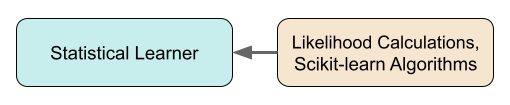
\includegraphics[width=0.7\linewidth]{./chapters/exp1/methodology3.png}
  \caption{Third portion of the flowchart from Figure \ref{fig:method} being 
           described in this section.}
\end{figure}

Choosing which algorithms to test is largely intuitive, but since this work has
yet to be benchmarked with simple algorithms, two straighforward algorithms
were chosen, \textit{k}-nearest neighbors and decision trees, and were
introduced in Section \ref{sec:algs}. Also covered in that section is the
mathematical framework of the \gls{MLL} calculation method. The implementation
details of these three approaches are covered here. 

\subsection{Scikit Algorithms}
\label{sec:scikit}

The machine learning toolkit chosen for this work is scikit-learn
\cite{scikit}, a package in python.  Virtually all modern \gls{ML} toolkits
will have acceptably fast and reliable algorithms, but the use of python
provides a platform for seamless integration of all the tools in the workflow. 

Prior to training, the data set is preprocessed by scaling and normalization
because the nuclide concentrations vary by many orders of magnitude. 

\subsection{Maximum Log-Likelihood Calculations}
\label{sec:mll}

The \gls{MLL} calculation method is implemented in python using the scipy 
statistics toolkit \cite{scipy}
